\begin{frame}[plain]\frametitle{}
\titlepage %表紙
\end{frame}


\begin{frame}\frametitle{紹介論文}
\begin{block}{[Su 15]}
\fullcite{Su2015}
\end{block}
\begin{itemize}
    \item 動画中の人物消去の検出タスク,精度 89\%
    \item K-SVD と K-Means を活用した動画特徴量抽出
    \item クラスタリングを活用した珍しい Video Forgery (VF) 研究
\end{itemize}
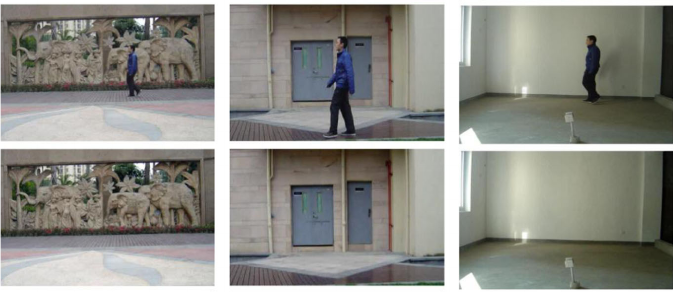
\includegraphics[scale=0.3]{figure/su.png}
\end{frame}


\begin{frame}\frametitle{候補だった論文 1/3}
\begin{block}{[Wang 15]}
``A Visual Model-Based Perceptual Image Hash for Content Authentication''
\cite{Wang2015}
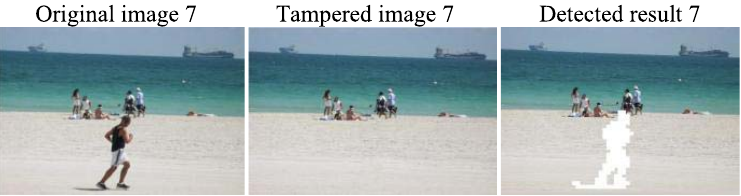
\includegraphics[height=1.5cm]{figure/wang0.png}
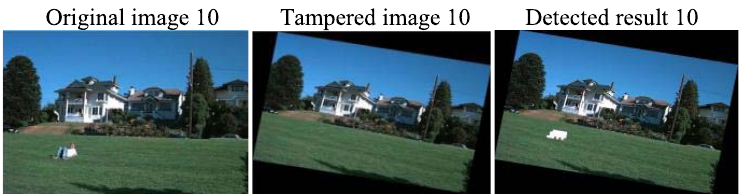
\includegraphics[height=1.5cm]{figure/wang1.png}
\end{block}
画像の認証・検索で有名な Perceptual Hash 特徴量の改良 \\
下記特徴量を compressive sensing でハッシュ列として統合
\begin{itemize}
    \item Keypoint based feature \\
        変形に頑健な SIFT の Wavelet 低周波成分
    \item Block based feature (改良点) \\
        内容に敏感な Watson's Visual Model (DCT) の低周波成分
\end{itemize}
\end{frame}


\begin{frame}{候補だった論文 2/3}
\begin{block}{[Chen 12]}
``Video Forgery Detection Based on Non-Subsampled Contourlet Transform and Gradient Information''
\cite{Chen2012}
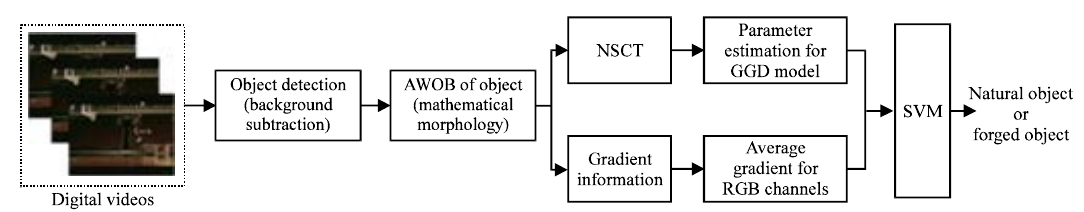
\includegraphics[height=2cm]{figure/chen0.png}
\end{block}
\begin{itemize}
    \item AWOB や NSCT という VF 検出で利用される特徴量の検討
    \item 手法の比較が微妙
\end{itemize}
\end{frame}


\begin{frame}{候補だった論文 3/3}
\begin{alertblock}{Video Inpainting系}
[Newson 14]\footfullcite{Newson2014}
[Granados 12]\footfullcite{Granados2012}
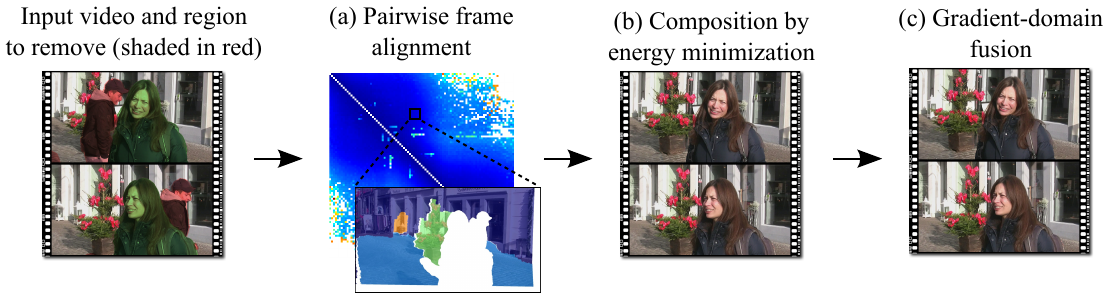
\includegraphics[height=2cm]{figure/granados.png}
\end{alertblock}
\begin{itemize}
    \item 映像中のマスク領域指定で人を自然に消す
    \item 彼らのサンプル(元動画 + マスク + 改ざん動画 + ソースコード)
    %\footnote{http://gvv.mpi-inf.mpg.de/projects/vidbginp}
    %\footnote{http://perso.telecom-paristech.fr/~gousseau/video_inpainting} 
    が Video Forgery の実験データセット作成に使えそう
\end{itemize}
\end{frame}


\begin{frame}{[Su 15] を選んだ理由}
修論は動画改ざん検出の研究をすることになった

\begin{itemize}
    \item VF 検出でフィルタバンク系の特徴量などが多い中,珍しく統計的な手法
    \item 他の研究では SVM など教師有り学習を行う中,識別も教師なし学習
    \item K-SVD (などスパース符号化) 関係の論文を読みたかった
\end{itemize}

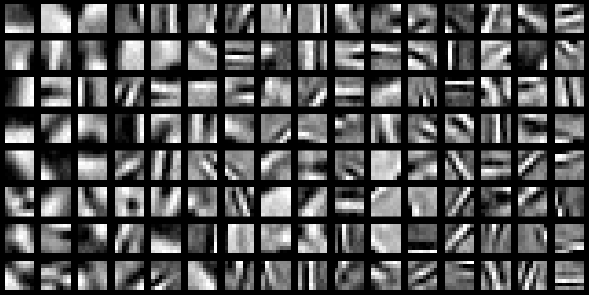
\includegraphics[height=2cm]{figure/ksvd.png}

画像から得られるK-SVD辞書の例\cite{Murata2012}
\end{frame}


\begin{frame}{TOC}
\tableofcontents
\end{frame}
